% Chapter Template

\chapter{Proposed Approach} % Main chapter title

\label{chapter4} % Change X to a consecutive number; for referencing this chapter elsewhere, use \ref{ChapterX}

\lhead{Chapter 4. \emph{Proposed Approach}} 

This section gives a detailed description of the implemented tracking system. Initially, giving an overview of the whole system and the basic functional blocks. Then, explaining implementation details of the different parts.

\section{The Tracking Loop}

Initially,  we explain the necessary building blocks of an object tracking system.

\section{Tracking system overview}

In order to tackle all the problems stated in the previous section, this tracking approach is separated into different modules.

\subsection{Basic overview}

Generic single-object tracking could be defined as the localization of an object through a video sequence. It is generic because the system is able to track any kind of object (faces, cars, etc.), and is single because the system will track just one object and not many at the same time. The proposed approach in this thesis is shown in \ref{fig::diagram}. Initially, our method starts with a pool of $n$ trackers $T = \left \{ t_1, t_2, ..., t_n \right \}$ and input data $\mathrm{x}$. This input corresponds to the initial rectangular box for an object in a sequence. All trackers are initalized and an updateable object model is created. Then, on each frame, our method runs and groups all trackers results by position into a set of $m$ clusters $C = \left \{ c_1, c_2, ..., c_m \right \}$. Also, we obtain a similarity measure which compares an actually tracking result patch to the current object model. The output should be the probabilities of similarity between the object model and each tracker result in that frame $S = \left \{ s_1, s_2, ..., s_n \right \}$. Using clustering information, the system can select between the winner cluster $c*$ which has the highest number of members, or the cluster with highest similarity measure. the others clusters are considered outliers and are reinitialized each 15 frames.

\begin{figure}[t!]
	\centering
		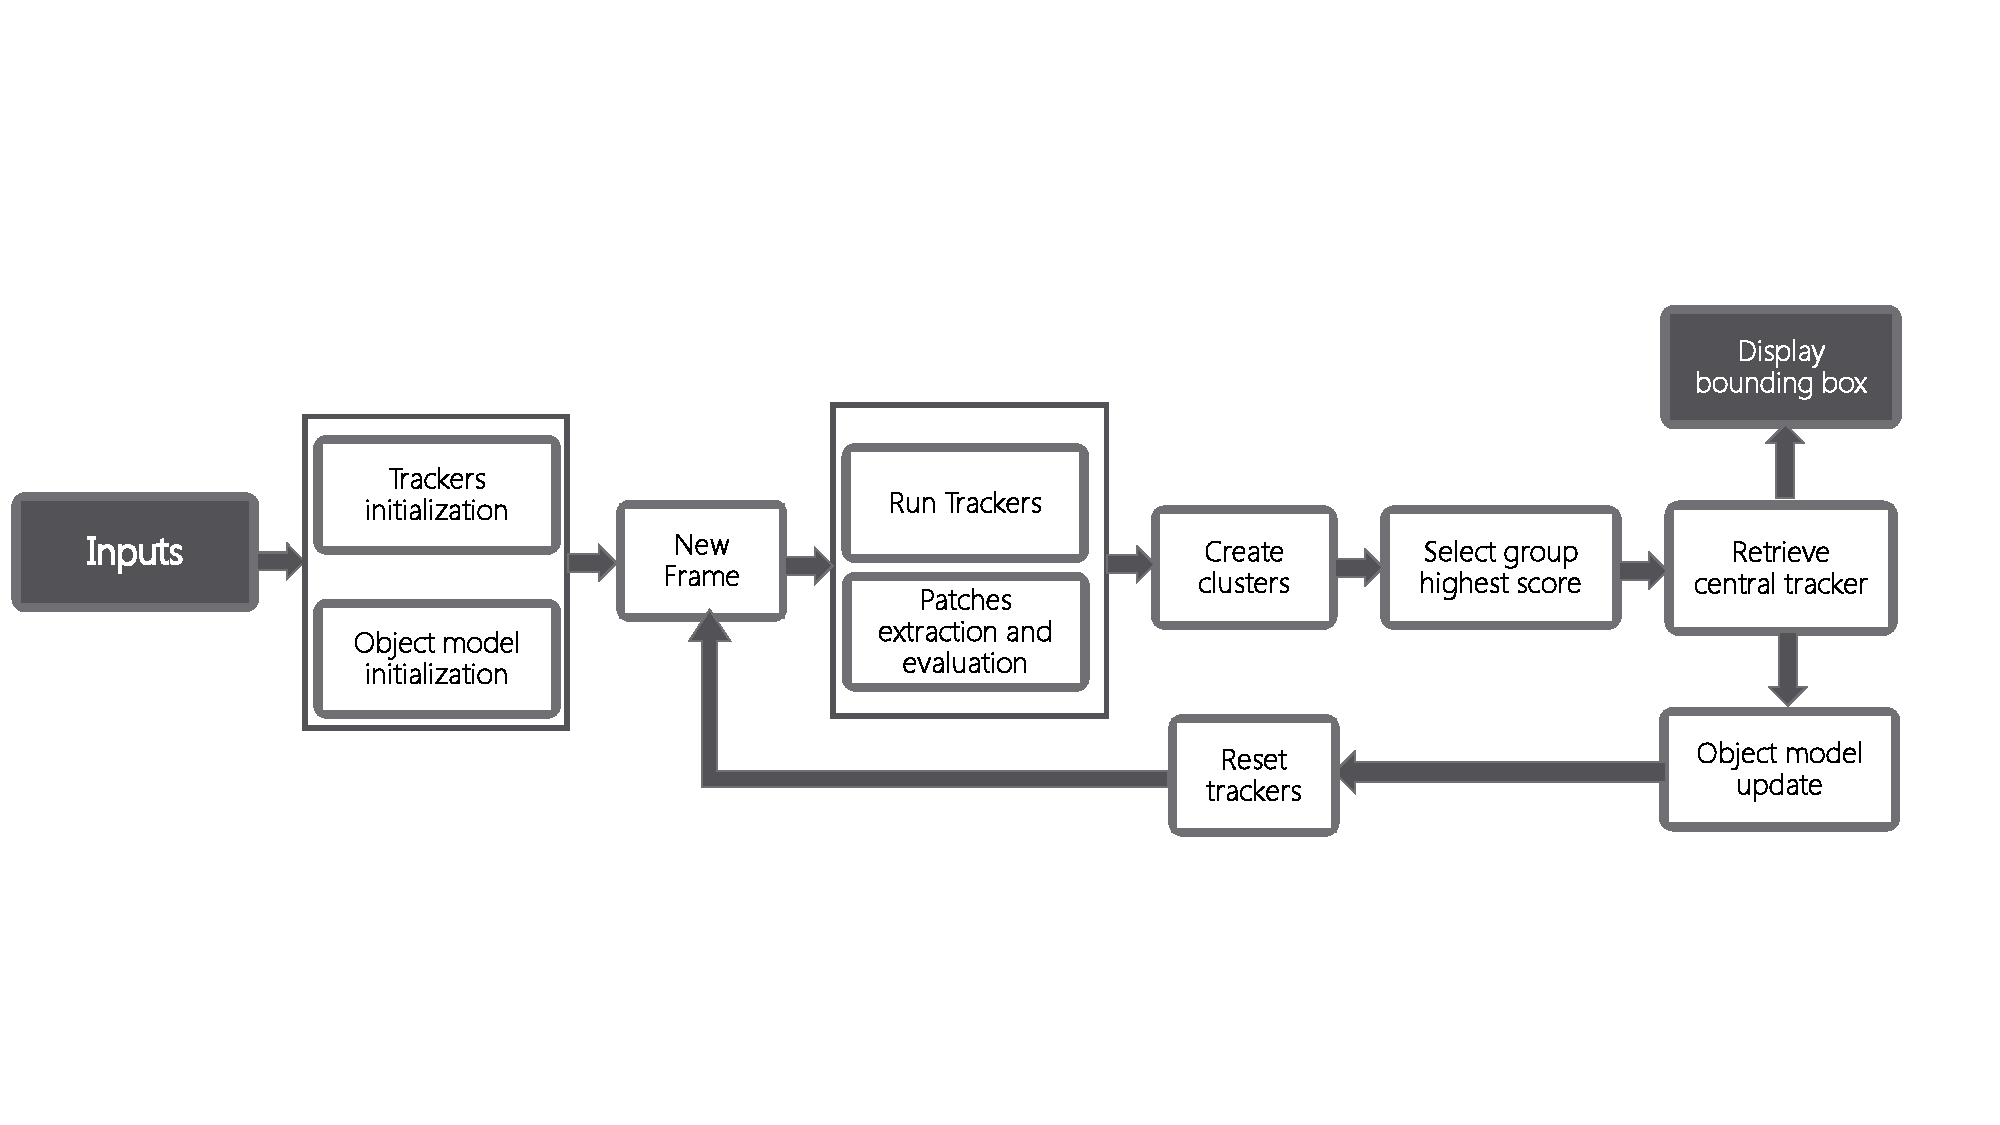
\includegraphics[width=1\linewidth, trim= 0cm 3cm 1cm 4cm, clip=true]{Figures/block_diagram.pdf}
	\caption{General schema for generic single-object tracking proposal.}
	\label{fig::diagram}
\end{figure}

\subsection{Trackers bounding boxes clustering}

Cluster analysis is the formal study of algorithms and methods for grouping, or classifying objects. These objects are described as a set of measurements or by relationships between the object and other objects. A \textit{cluster} is comprised of a number of similar objects collected or group together. Other authors define a cluster as a set of entities which are alike, and entities from different clusters are not alike, or "A cluster is an aggregation of points in the test space such that the \textit{distance} between any two points in the cluster is less than the distance between any point in the cluster and any point not in it". This theory is taken from \textbf{Jane and Dubes.}

Cluster analysis is the process of classifying objects into subsets that have meaning in the context of a particular problem. The objects are thereby organized into an efficient representation that characterizes the data. Clustering methods require that an index of proximity, or alikeness, or affinity, or association be established between pairs or patterns. A \textit{proximity matrix} $|d(i, j)|$ accumulates the pairwise indices of proximity in a matrix in which each row and column represents a pattern. Diagonal entries of a proximity matrix are ignored since all paterns are assumed to have the same degree of proximity with themselves. Also it is assmed that all proximity matrices are symmetric, so all pairs of objects have the same proximity index, independent of the order in which they are written.

A proximity index is either a \textit{similarity} or a \textit{dissimilarity}. The more the \textit{i}th and \textit{j}th objects are similar one another, the larger a similarity index and the dissimilarity index are.

Previous works show the common approach of data fusion using majority voting. The authors in \cite{Bailer2013} applied this method using a threshold parameter that defines if two result boxes vote for the same position. However, in \cite{Bailer2014}, the authors proved that this approach is sequence dependent. Instead, they settle the idea of attraction fields. We base our approach using the idea of clustering position. On a new frame, each tracker will give a rectangular box of where the object might be. Using this information, we are able to form groups of trackers that have similar positions. For each tracker result, we calculate the distance between its position and the rest of trackers running. The distance $d$ between two boxes $b$ and $c$ is computed as:

\begin{equation}
\large
d(b,c) = 1 - \frac{b\bigcap c}{b\bigcup  c}
\end{equation}

Using all distances, we construct a symmetric $l \times l$ proximity matrix $D$. We take the proximities to be dissimilarities. This means that $d(i,i) = 0$ for all $i$. We use complete-link hierarchical agglomerative clustering to form groups of trackers. Trackers $t_1$ and $t_2$ are "related" if their dissimilarity is below some threshold $v$. CL merges clusters in order of proximity; the closest clusters will be merged first, and the furthest clusters will be merged last. At each merge, CL creates a \textit{reduced proximity matrix}, with one less row and column. At the end, the algorithm delivers a set of clusters with size $m$ $C = \left \{ c_1, c_2, ..., c_m \right \}$ satisfying the following:
\begin{itemize}
\item $c_i \cap c_j = \emptyset$ for $i$ and $j$ from 1 to $m$, $i \neq j$
\item $c_1 \cup c_2 \cup ... \cup c_m = T$
\end{itemize}

\begin{figure}[t!]
	\centering
		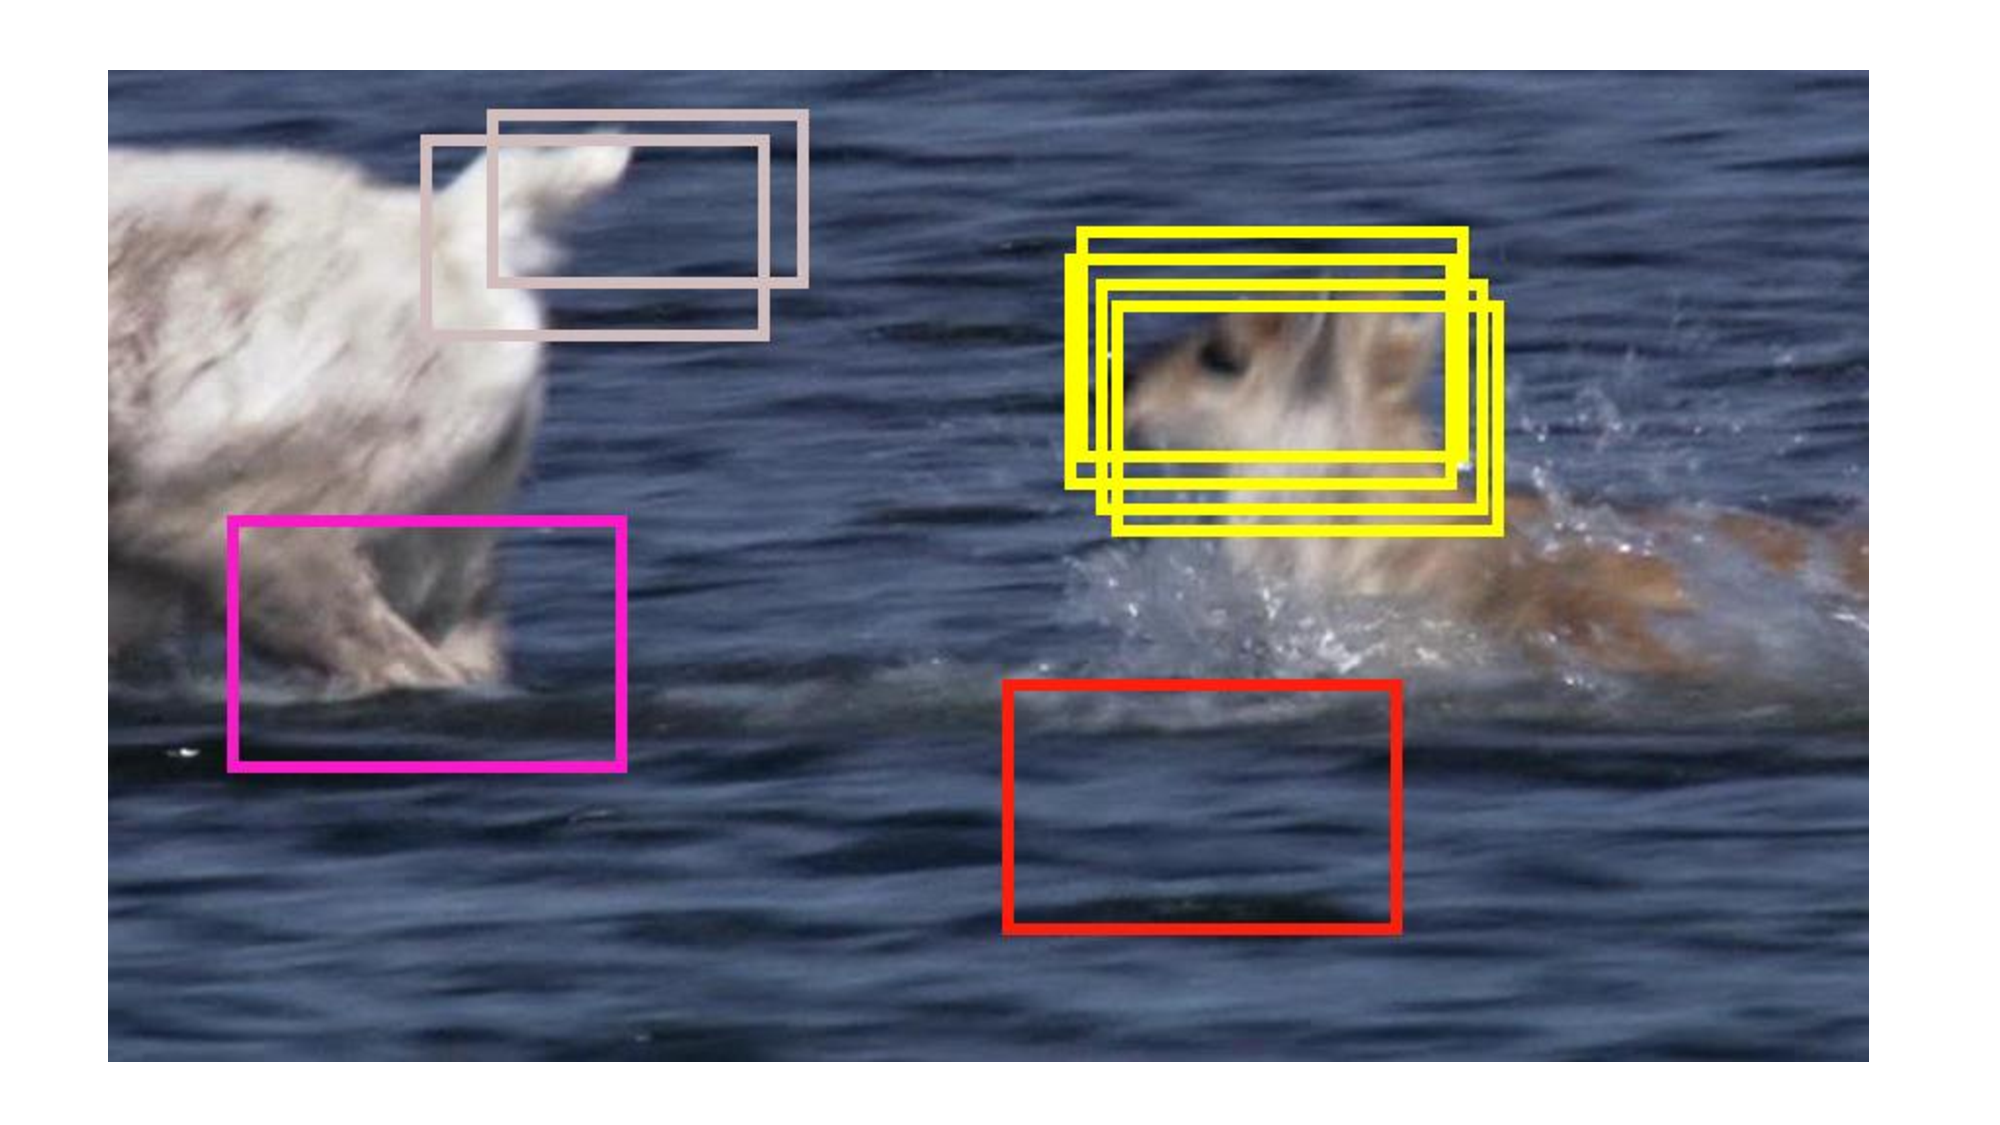
\includegraphics[width=0.65\linewidth, trim= 1cm 1cm 1cm 1cm, clip=true]{Figures/trackers_clustering.pdf}
	\caption{Tracking results clustering.}
	\label{fig::trackers_clustering}
\end{figure}

\subsection{Object modeling}

Visual object tracking has been formulated as a tracking-by-detection problem recently. In this case, object modeling is dynamically performed to support object detection in all frames. Mostly all approaches can be classified into two categories: \textit{Generative appearance models}, that mainly focus on how fit data into their correspondent object class; and \textit{discriminative appearance models}, that assume object tracking as a binary classification issue. The main goal is to maximize the separability between object and non-object regions discriminately.

Generally, Discriminative methods train a classifier using data acquired from previous frames, and subsequently use the trained classifier to evaluate possible object regions at the current frame (Figure \ref{fig::svm_example}). After localization, a set of \textit{positive} and \textit{negative} samples are heuristically selected to update the classifier. Some approaches apply online boosting \textbf{Cites}, that make a discriminative evaluation of features taken from a candidate feature pool, and then select the top ranked features to conduct the tracking process. Other methods apply Support Vector Nachines (SVM) method, which learns a margin-based discriminative appearance model, in order to maximize inter-class separability. It is important to note that these classifiers are trained using visual representations of the object.

\begin{figure}[t!]
		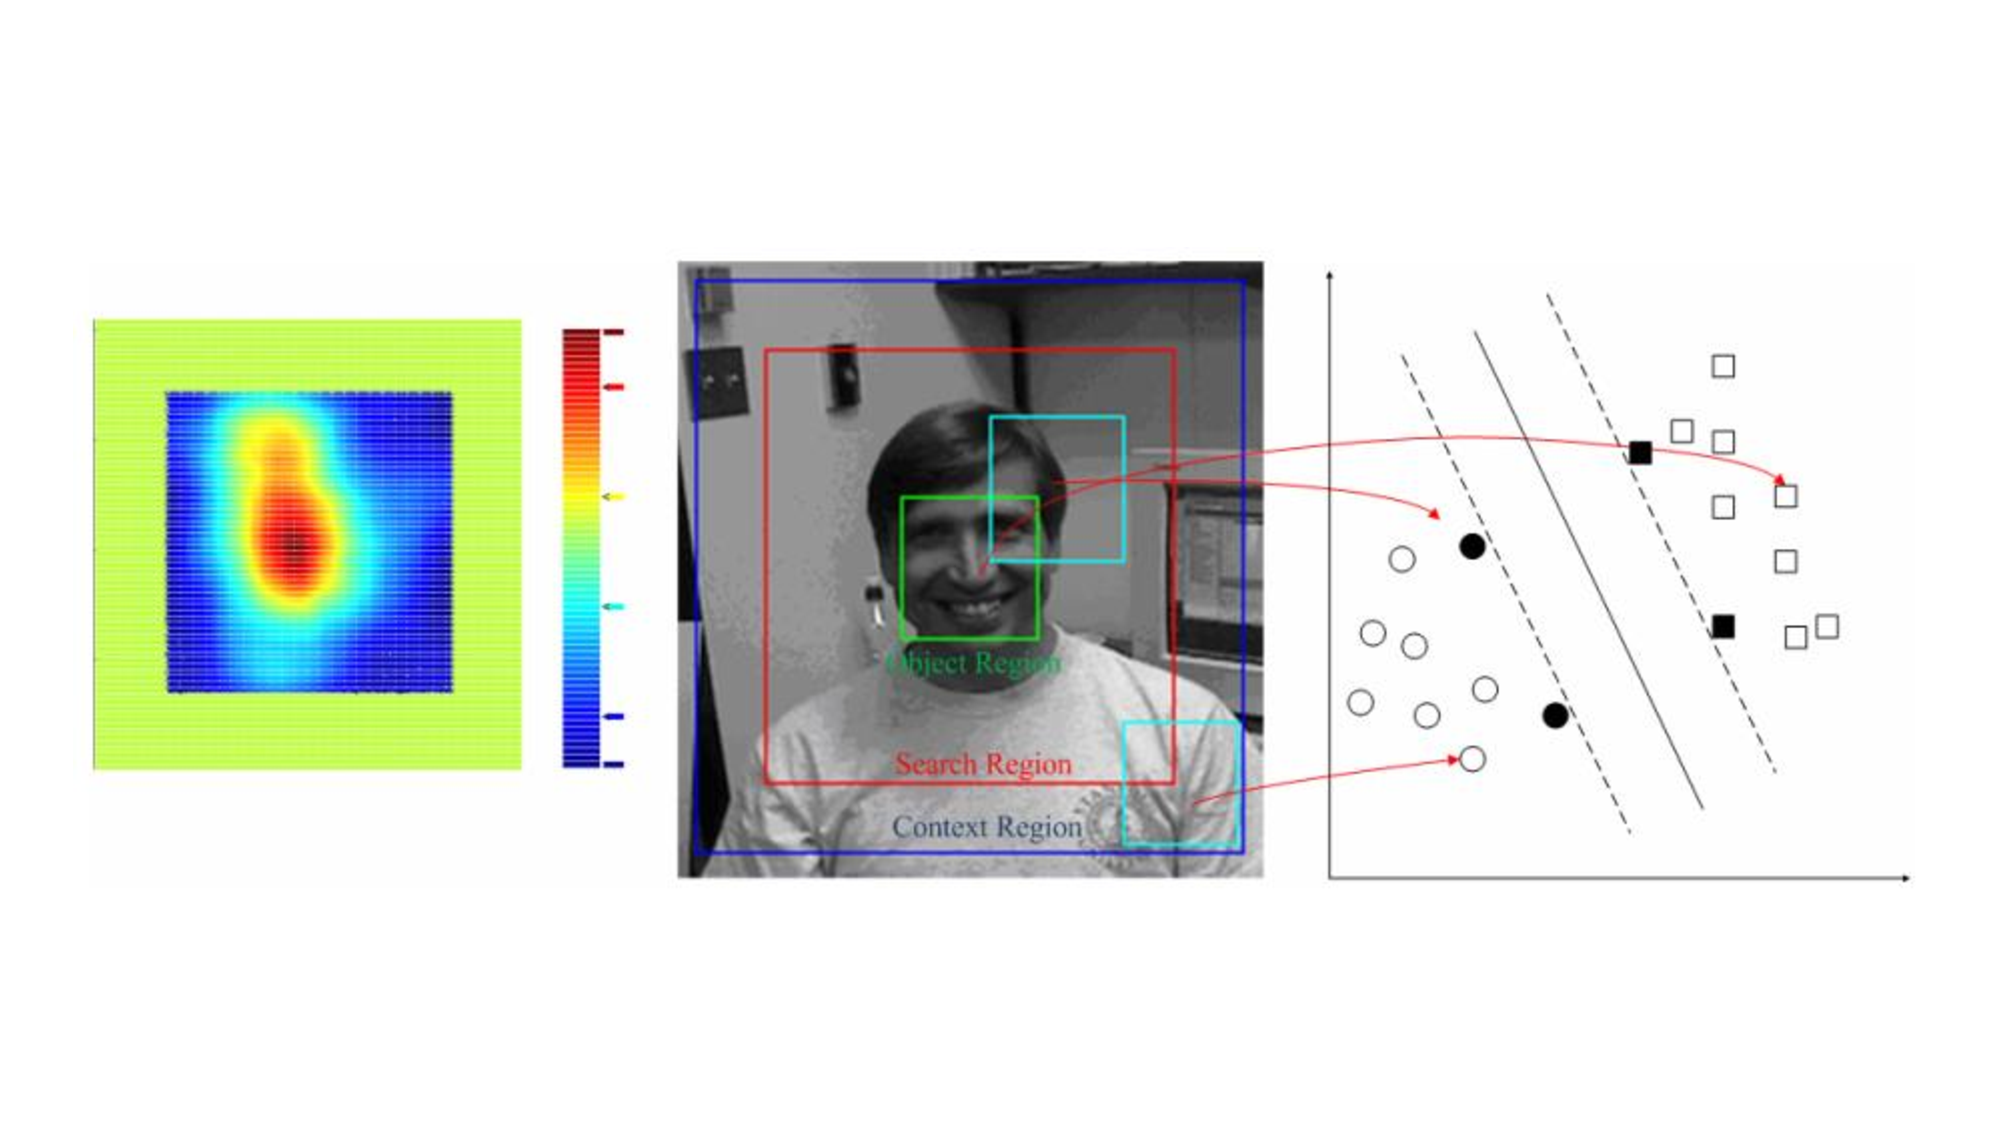
\includegraphics[width=1\linewidth, trim= 0cm 3cm 1cm 4cm, clip=true]{Figures/svm_example.pdf}
	\caption{Example of tracking-by-detection approach based on SVM classification. The left subfigure shows the score map of face and non-face classification; middle subfigure shows the search region for object localization and the context region for face and non-face samples selection; right subfigure plots the classification hyperplane that separates face and non-face classes.}
	\label{fig::svm_example}
\end{figure}


Tracking methods applying object appearence online learning have been recently applied. These systems discriminate object from its surrounding background through all the sequence using a classifier updated based on tracking results. However, these approaches except for MILBoost \cite{Babenko2010}, suffer from label jitter. The authors in \cite{Santner2010} explain that problem of label jitter arises if the bounding boxes of an object are not perfectly aligned with the target, although it is detected correctly. If label jitter occurs repeatedly over a tracking sequence, the tracker will most likely start to lose the target object. To cope this problem, we consider selecting a bag of trackers which share common similarity with appearance model.

The classifier corresponds to a standard linear SVM, which is trained with a buffer of 10 positives and 100 negative examples. The positive buffer is initialized using $\mathrm{x}$. We extract and image patch and calculate hog features. For the negative buffer we sample random bounding boxes with the same size on the image. During tracking, whenever a new example is added to the buffer, the classifier is retrained.


\subsection{Best cluster selection}

After perfoming clustering stage and obtaining classification scores with each tracker results, we can select the cluster that best follows the object. We present two selection criterias for best cluster.

\textbf{Best cluster selection based on members criteria:} Once groups are formed, we search the cluster $c^{*}$ in the list of clusters $C$ of size $m$, with highest number of trackers.

\begin{equation}
\large
c^{*} = \arg\max_{c\in C} ~\sum_{t \in c}t_{i} 
\end{equation}

\textbf{Best cluster selection based on appearance scores:} In this case we are considering classification scores for each cluster. Each cluster gives a score per cluster. Then, we select the winner cluster whose score is the highest one. 
\begin{equation}
\large
c^{*} = \arg\max_{c\in C} m_{i}
\end{equation}

where $m_i \in M = \left \{ m_1, m_2, ..., m_m \right \}$ corresponds to maximum score value of $c_i$ cluster:

\begin{equation}
\large
M =  \left \{ \max_{s\in S} s_i \in c_i \right \}
\end{equation}


\subsection{Best tracker selection}

The centered position $\mathrm{x}^{*}$ is selected by choosing the minimum sum of distances of the tracker, to the rest of trackers that belong to $c^{*}$. We did not consider selecting the tracker with best appearance score in order to avoid label jitter and drifting problems. Also selecting this value might make the tracker shaky.

\begin{equation}
\large
\mathrm{x}^{*} = \arg\min_{\mathrm{x}} ~\sum_{\mathrm{x}_{i} \in w^{*}}d(\mathrm{x_{i}}, \mathrm{x_{j}}) ,~~ i \neq j, \mathrm{x_{j}}\in c^{*}
\end{equation}

\begin{figure}[t!]
	\centering
		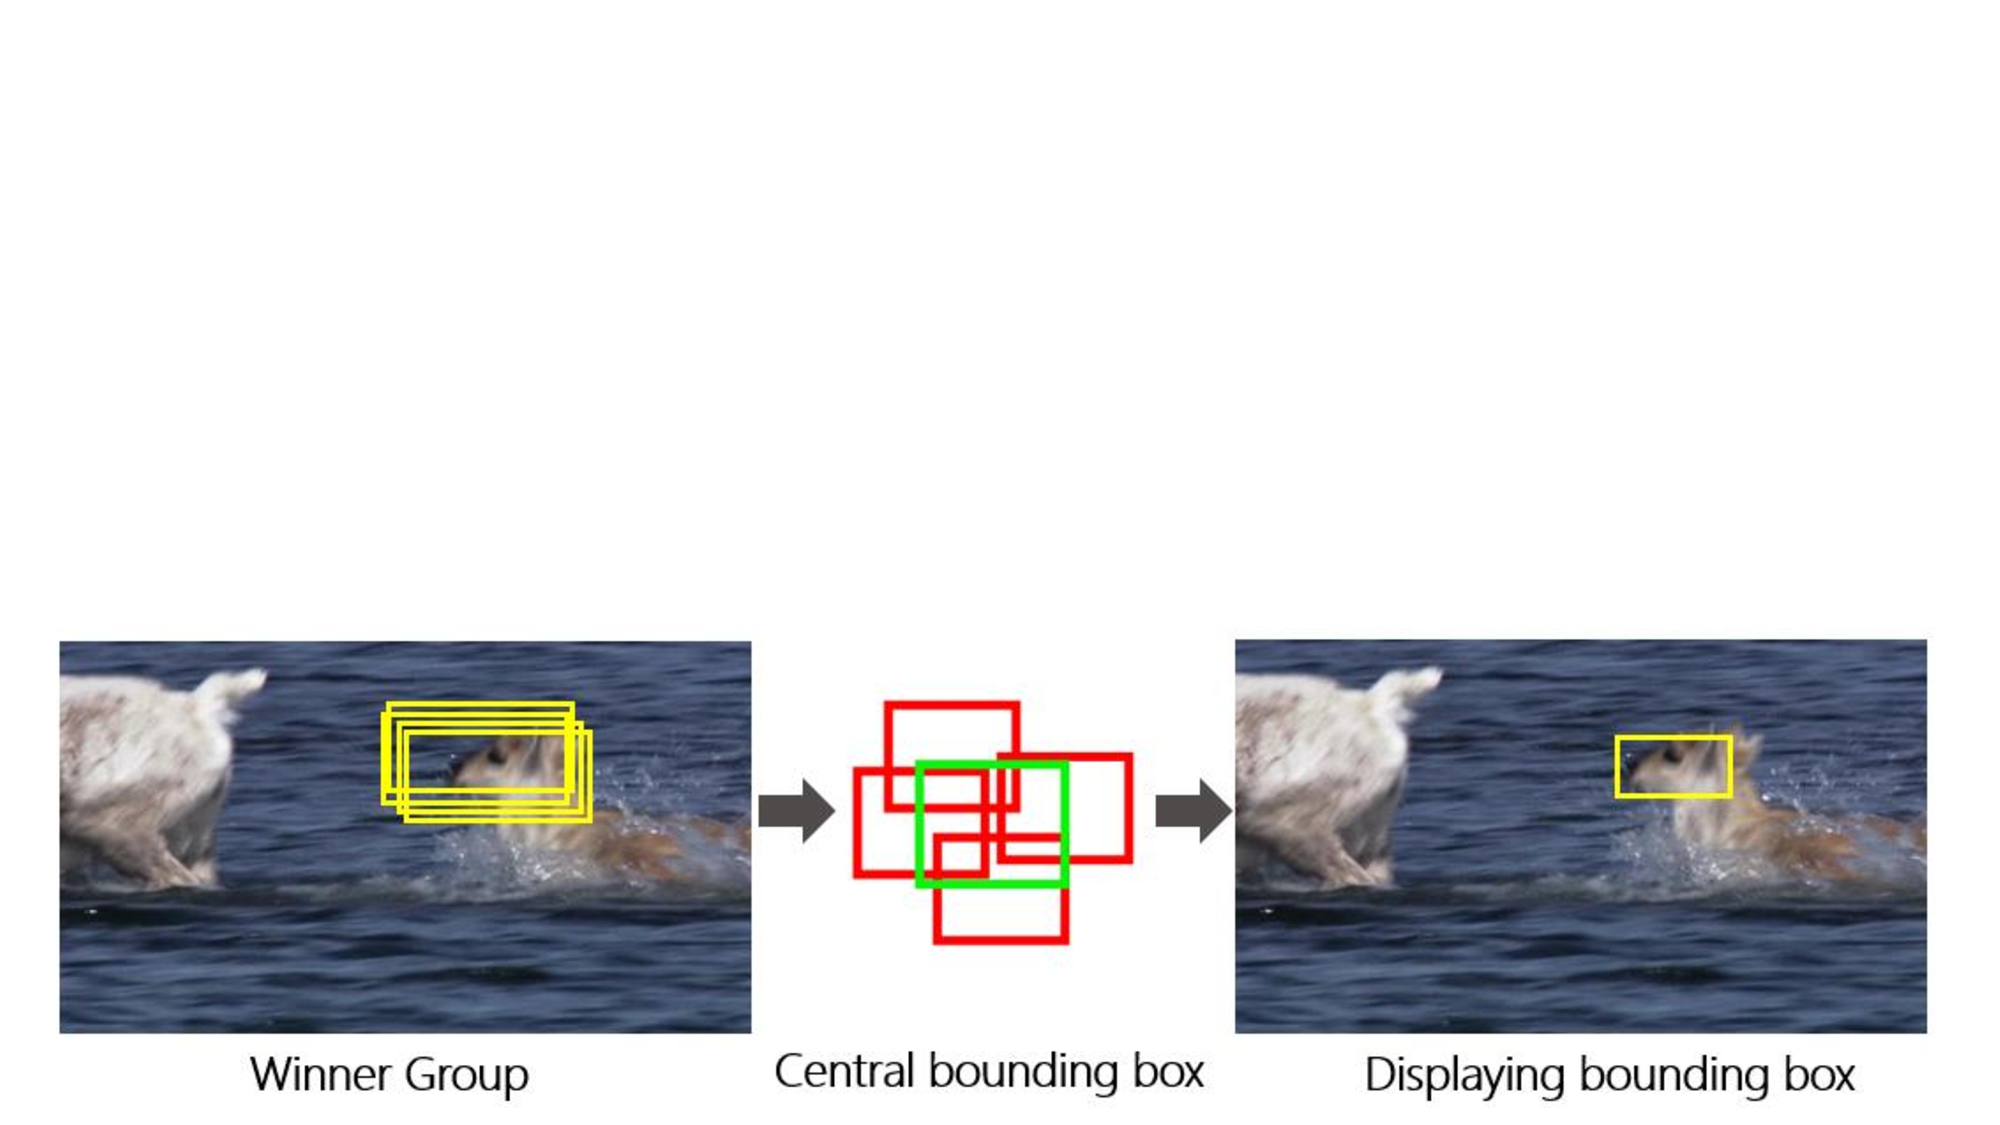
\includegraphics[width=0.95\linewidth, trim= 1cm 0cm 1cm 11cm, clip=true]{Figures/best_tracker.pdf}
	\caption{Best tracker bounding box selection.}
	\label{fig::best_tracker}
\end{figure}



\subsection{Trackers reset}

The outliers correspond to those trackers that does not belong to $c^*$. These trackers are reinitialized using $\mathrm{x}^{*}$. Also, from $\mathrm{x}^{*}$, we crop and image patch and extract hog features as new positive sample for the classifier.

\begin{equation}
\large
R = t_i \not\subset c^*
\end{equation}

\subsection{Object model update}
